
\begin{center}
\Huge
Opgaver i potensfunktioner
\end{center}
\section*{Opgave 1}
\stepcounter{section}

I Fig. \ref{fig:potensfunktioner} er fire potensfunktioner givet. Deres forskrifter er 
\begin{align*}
f(x) &= \frac{1}{2}\cdot x^2,\\
g(x) &= 2\cdot x^{\frac{1}{3}},\\
h(x) &= x,\\
l(x) &= 2\cdot x^{-1}.
\end{align*}
Par disse funktioner med graferne fra Fig. \ref{fig:potensfunktioner}. Begrund dit svar.
\begin{figure}[H]
\centering
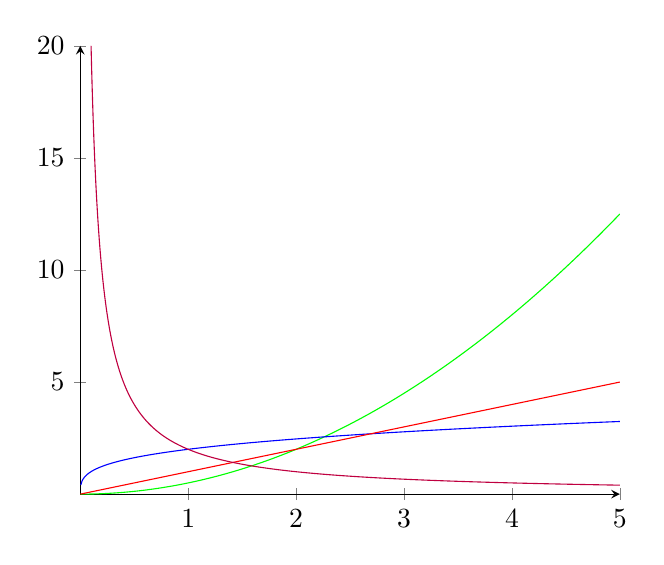
\begin{tikzpicture}
\begin{axis}[ axis lines = middle, xmin = 0, xmax = 5
]
\addplot[samples = 1000, color = green] {0.5*x^2};
\addplot[samples = 1000, color = blue] {2*x^0.3};
\addplot[samples = 1000, color = red] {x};
\addplot[samples = 1000, color = purple, domain = 0.1:5] {2*x^(-1)};
\end{axis}
\end{tikzpicture}
\caption{Grafer for fire potensfunktioner}
\label{fig:potensfunktioner}
\end{figure}

\section*{Opgave 2}
\begin{enumerate}[label=\roman*)]
\item En potensfunktion $f(x) = 4\cdot x^a$ går gennem punktet $(2,16)$. Brug dette til at bestemme $a$.
\item En potensfunktion $g(x) = b\cdot x^a$ går gennem punkterne $(1,3)$ og $(2,8)$. Brug dette til at bestemme $a$ og $b$.
\item En potensfunktion $h(x) = b\cdot x^3$ går gennem punktet $(1,1)$. Brug dette til at bestemme $b$. 
\end{enumerate}
\section*{Opgave 3}
Følgende datasæt er givet:
\begin{center}
\begin{tabular}{c|c|c|c|c|c|c}
$x$& 0.3 & 0.6 & 0.9 & 1.2 & 1.5 & 1.8\\\hline
$y$ & 1 & 1.2 & 1.9 & 1.7 & 2.3 & 3.3\\
\end{tabular}
\end{center}
\begin{enumerate}[label=\roman*)]
\item Bestem den potensfunktion, der bedst beskriver datasættet.
\item Bestem den lineære funktion, der bedst beskriver datasættet. 
\item Det oplyses, at det næste punkt i datasættet er $(2.1,4.2)$. Er det den lineære model eller potensmodellen, der bedst rammer dette punkt?
\end{enumerate}

\section*{Opgave 4}
\begin{enumerate}[label=\roman*)]
\item For en potensfunktion $f(x) = b\cdot x^2$ øger vi $x$ med $50\%$. Hvor meget øger vi $f(x)$ med?
\item En potensfunktion $f(x)$ går gennem punkterne $(2,3)$ og $(4,10)$. Vi øger $x$ med $15\%$. Hvor meget øges $f(x)$ med?
\end{enumerate}
\section*{Opgave 5}
Bremselængden for en bil kan beskrives ved $D$ givet ved
\begin{align*}
D(v) = k\cdot v^2.
\end{align*}
\begin{enumerate}[label=\roman*)]
\item Hvis vi øger hastigheden med $20\%$, hvor meget øges bremselængden $D$ så med?
\item Hvis vi vil sænke vores bremselængde med $50\%$, hvor meget skal vi så sænke vores hastighed med?
\end{enumerate}

\section*{Opgave 6}
Bevis topunktsformlen for potensfunktioner, ved at bruge $\ln$ i stedet for $\log$.